\lstinputlisting[language=bash,basicstyle=\small]{python_codes/fieldstone_101/keywords.ascii}

\begin{center}
Code at \url{https://github.com/cedrict/fieldstone/tree/master/python_codes/fieldstone_101}
\end{center}

\par\noindent\rule{\textwidth}{0.4pt}

%%%%%%%%%%%%%%%%%%%%%%%%%%%%%%%%%%%%%%%%%%%%%%%%%%%%%%%%%%%%%%%%%%%%%%%%%%%%%%%%%%%%%%%%%%%%%%%%%%%%

\begin{center}
\includegraphics[width=1cm]{images/fortran/fortran} 
\end{center}

This stone explores the possibilities offered by the Y12M direct solver\footnote{
\url{http://www.netlib.org/y12m/doc}}. It is identical 
to \stone~01. Despite its age (it was published in 1981), 
this solver remains interesting because it is rather compact, has a simple interface, fits in 
a single file and relies on a sparse storage for the FE matrix.

The documentation \cite{zlws81} states:
"The Y12M is a package of Fortran subroutines for the solution of large and sparse systems of
linear algebraic equations developed at the Regional Computing Centre at the University of
Copenhagen (RECKU). Gaussian elimination and pivotal interchanges are used to factorize
the matrix of the system into two triangular matrices L and U. An attempt to control the
magnitude of the non-zero elements in order to avoid overflows or underflows and to detect
singularities is carried out during the process of factorization, lterative refinement of the first
solution may be performed. It is verified (by a large set of numerical examples) that iterative
refinement combined with a large drop-tolerance and a large stability factor is often very
successful when the matrix of the system is sparse, Not only is the accuracy improved but
the factorization time is also considerably reduced so that the total computing time for the
solution of the system with iterative refinement is less than that without iterative refinement
(in some examples the total computing time was reduced by more than three times). The
storage needed can often be reduced also."

The Y12M solver comes in two versions Y12MAE (single precision) and Y12MAF (double precision).
We obviously use the latter in the code. 
This solver requires the matrix to be stored in COO coordinates, not CSR nor CSC.
The non-zero entries are then stored in two integer arrays SNR and RNR of length Nfem:
\begin{itemize}
\item SNR - INTEGER array. On entry SNR(j) must contain the
column number of the non-zero element stored in A(j).
The content of array SNR is modified by
subroutine Y12MA. 
\item RNR - INTEGER array. On entry RNR(i) must contain the row
number of the non-zero element stored in A(i).
The content of array RNR is modified by subroutine Y12MA.
\end{itemize}
Note that since I had the code for building the CSR arrays I build these and use them to fill SNR and RNR:
\begin{lstlisting}[language=Fortran]
nz=0
snr(1)=1
rnr(1)=1
ia(1)=1
do j1=1,nny
do i1=1,nnx
   ip=(j1-1)*nnx+i1 ! node number
   do k=1,ndof
      ii=2*(ip-1) + k ! address in the matrix
      nsees=0
      do j2=-1,1 ! exploring neighbouring nodes
      do i2=-1,1
         i=i1+i2
         j=j1+j2
         if (i>=1 .and. i<= nnx .and. j>=1 .and. j<=nny) then ! if node exists
            jp=(j-1)*nnx+i  ! node number of neighbour 
            do l=1,ndof
               jj=2*(jp-1)+l  ! address in the matrix
               nz=nz+1
               snr(nz)=ii
               rnr(nz)=jj
               ja(nz)=jj
               nsees=nsees+1
            end do
         end if
      end do
      end do
      ia(ii+1)=ia(ii)+nsees
   end do ! loop over ndofs
end do
end do
\end{lstlisting}
This algorithm only works when the mesh is structured and linear elements are used. Also, 
despite the matrix being symmetric it must be stored in its entirety here. 

The code can be compiled by means of the {\filenamefont compile} script (you may need to 
modify it to make it compatible with your machine) and the code is executed by running
the generated {\filenamefont simplefem} executable.  

There is a built-in loop in the code which varies resolutions from $8\times 8$ to $256\times 256$.
We can then look at the solve time as a function of velocity degrees of freedom: 

\begin{center}
\includegraphics[width=10cm]{python_codes/fieldstone_101/results/timings.pdf}
\end{center}

It carries out a solve on a $256\times 256$ mesh in about 130s. This is of course rather slow when compared to 
MUMPS performance, but it allows for plenty of testing.
The code also computes the root mean square velocity and we can see that it becomes more and more accurate with 
an increase in resolution (i.e. a decrease in element size $h$), which is also confirmed by looking at the 
velocity error convergence, found to be quadratic as expected (see \stone 1):

\begin{center}
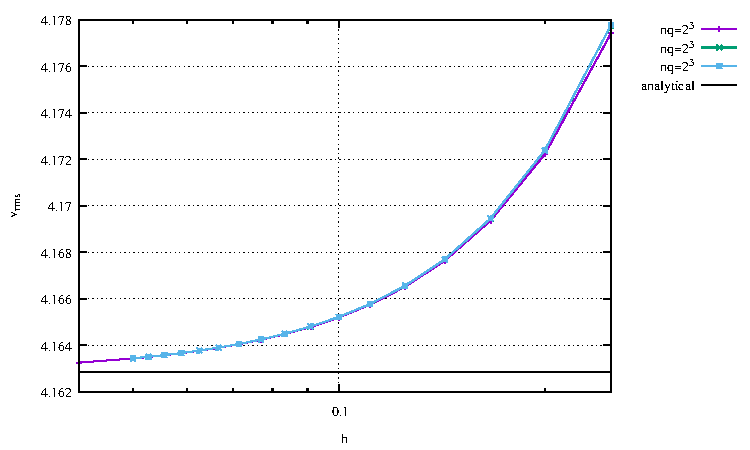
\includegraphics[width=7cm]{python_codes/fieldstone_101/results/vrms.pdf}
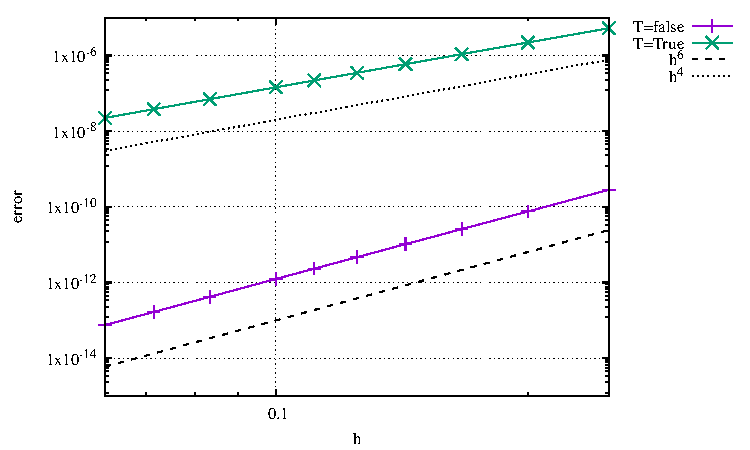
\includegraphics[width=7cm]{python_codes/fieldstone_101/results/errv.pdf}
\end{center}


